\documentclass[margin=5mm]{standalone}% For the example only, any class will do

\usepackage{tikz}
\usetikzlibrary{shapes.misc, positioning, arrows}

\usepackage{graphics}
%\pgfrealjobname{hierarchy}

\definecolor{blue}{HTML}{6363FF}
\definecolor{lightblue}{HTML}{87CEFA}
\definecolor{darkgreen}{HTML}{307430}
\definecolor{green}{HTML}{20A020}
\definecolor{lightgreen}{HTML}{00FF00}

\definecolor{yellow}{HTML}{FFFF00}
\definecolor{orange}{HTML}{FFA500}
\definecolor{lightred}{HTML}{EC5F5F}
\definecolor{red}{HTML}{CD1818}
\begin{document}
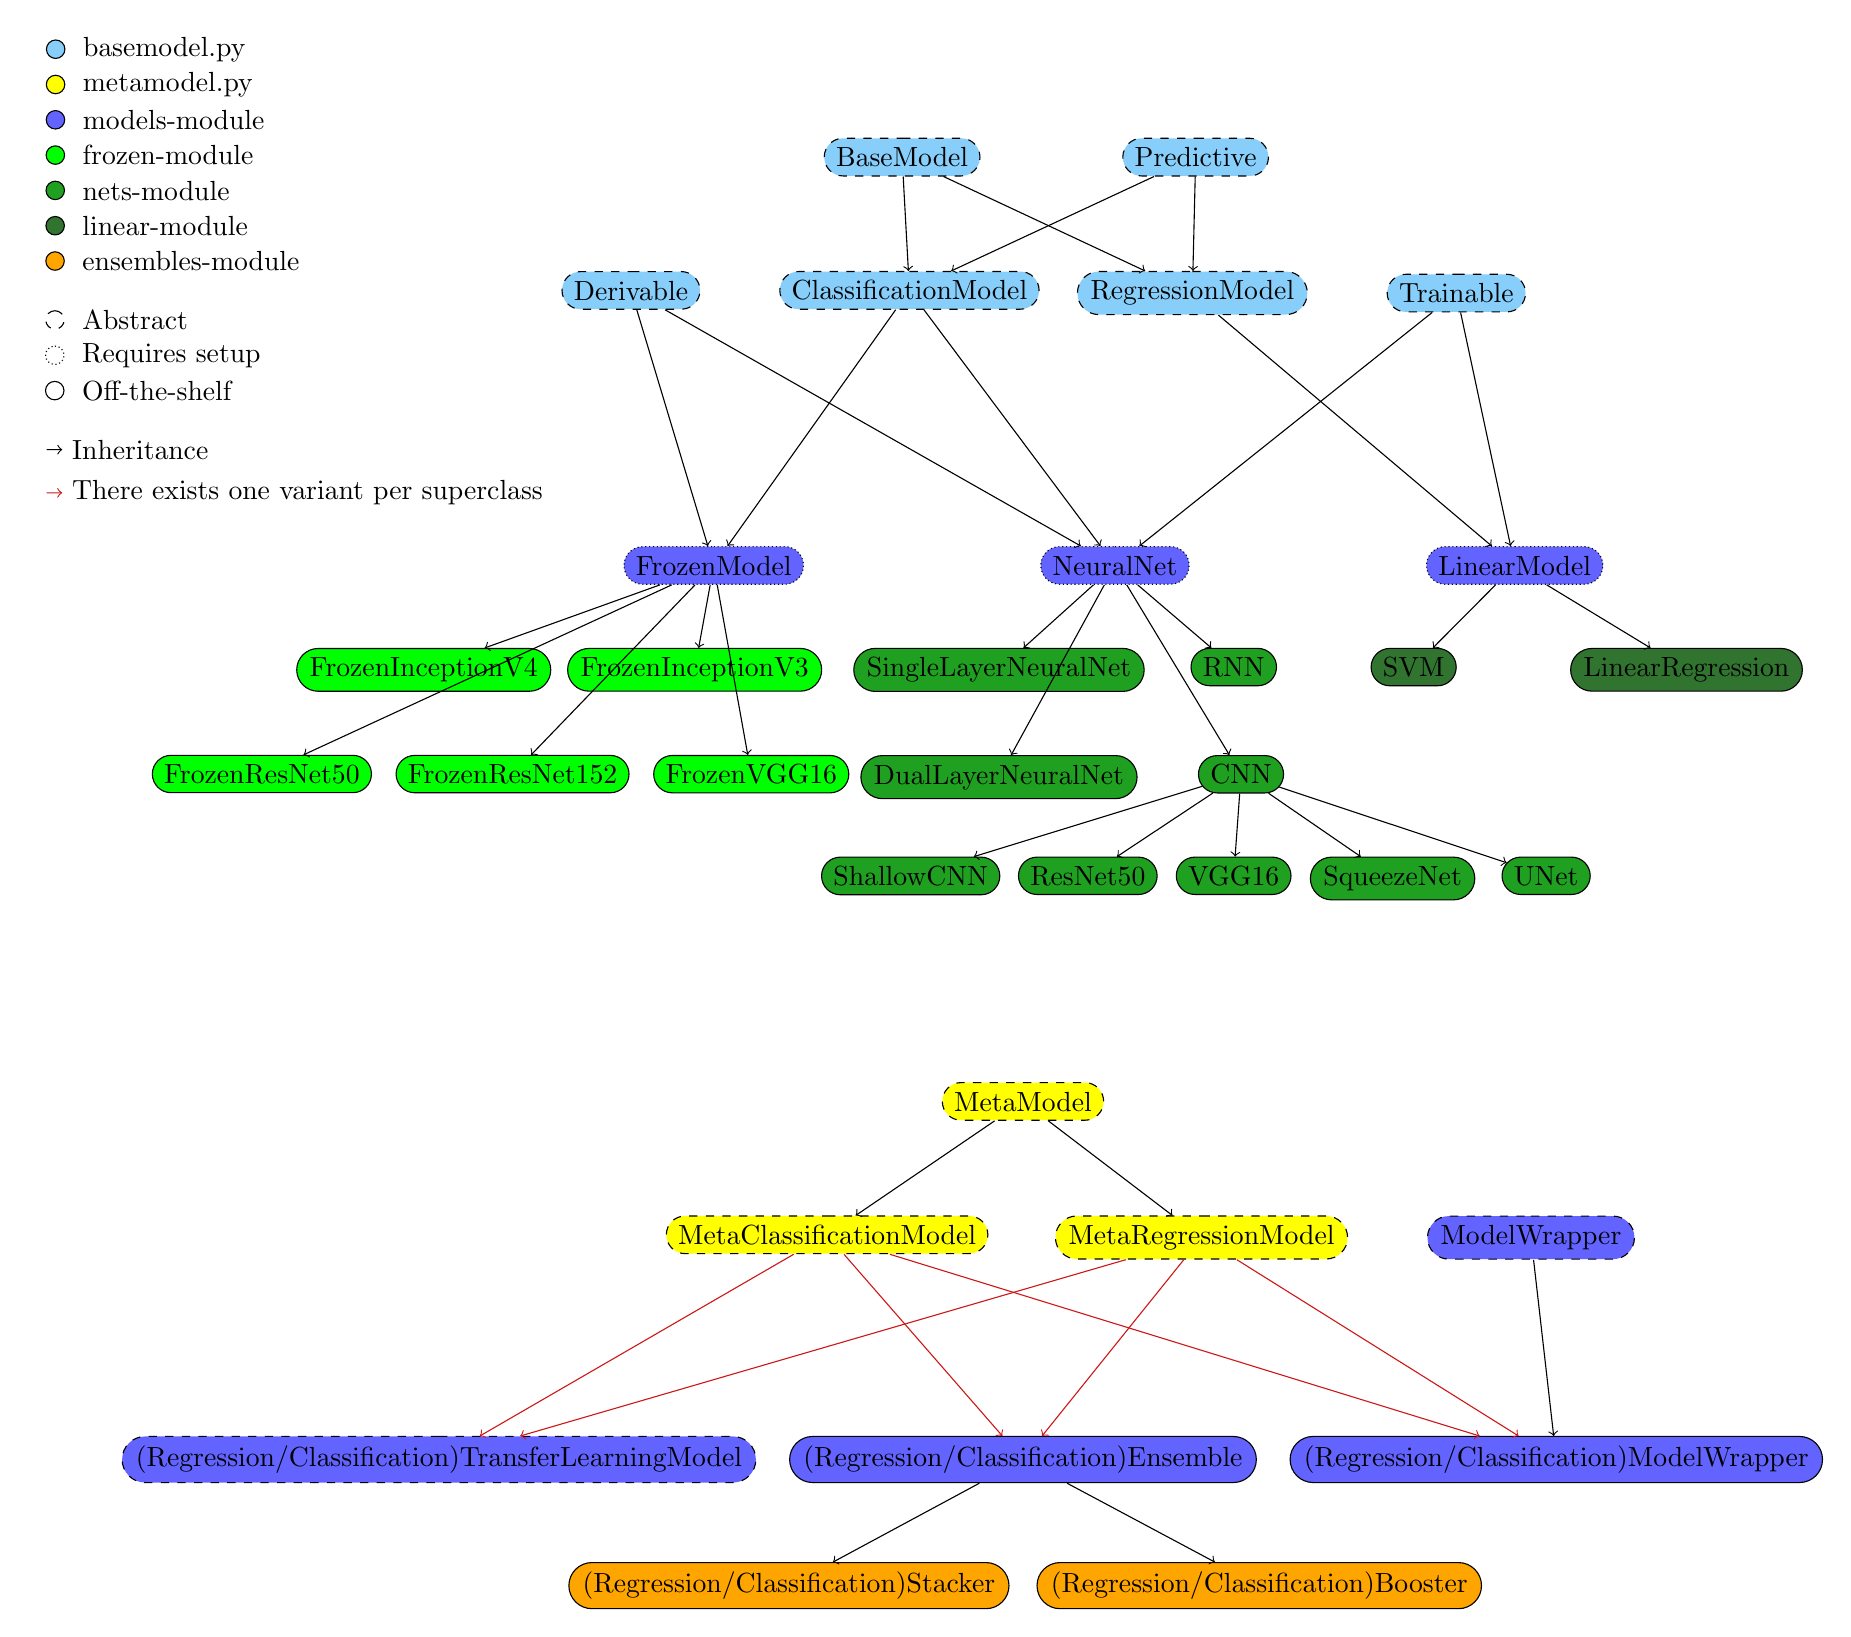
\begin{tikzpicture}[scale=1.5]
    \node (basemodel) [draw, dashed, fill=lightblue, rounded rectangle] {BaseModel};
    \node (predictive) [right=1.8cm of basemodel, draw, dashed, fill=lightblue, rounded rectangle] {Predictive};
    \node (predclassification) [below left=1.2cm and -2.25cm of basemodel, draw, dashed, fill=lightblue, rounded rectangle] {ClassificationModel};
    \node (predregression) [below right=1.2cm and 1.75cm of basemodel, draw, dashed, fill=lightblue, rounded rectangle] {RegressionModel};
    \node (trainable) [right=of predregression, draw, dashed, fill=lightblue, rounded rectangle] {Trainable};
    \node (derivable) [left=of predclassification, draw, dashed, fill=lightblue, rounded rectangle] {Derivable};

    \node (nn) [below right=3cm and 0.5cm of predclassification, draw, densely dotted, fill=blue, rounded rectangle] {NeuralNet};
    \node (singlenn) [below left=0.8cm and -0.8cm of nn, draw, fill=green, rounded rectangle] {SingleLayerNeuralNet};
    \node (dualnn) [below=0.8cm of singlenn, draw, fill=green, rounded rectangle] {DualLayerNeuralNet};
    \node (rnn) [below right=0.8cm and 0.5cm of nn, draw, fill=green, rounded rectangle] {RNN};
    \node (cnn) [below right=0.8cm and 1.2 of singlenn, draw, fill=green, rounded rectangle] {CNN};
    \node (shallow) [below left=0.8cm and 3cm of cnn, draw, fill=green, rounded rectangle] {ShallowCNN};
    \node (resnet50) [below left=0.8cm and 1cm of cnn, draw, fill=green, rounded rectangle] {ResNet50};
    \node (vgg16) [below left=0.8cm and -0.7cm of cnn, draw, fill=green, rounded rectangle] {VGG16};
    \node (squeeze) [below left=0.8cm and -3cm of cnn, draw, fill=green, rounded rectangle] {SqueezeNet};
    \node (unet) [below left=0.8cm and -4.5cm of cnn, draw, fill=green, rounded rectangle] {UNet};

    \node (linear) [right=3cm of nn, draw, densely dotted, fill=blue, rounded rectangle] {LinearModel};
    \node (linreg) [below right=0.8cm and 0.1cm of linear, draw, fill=darkgreen, rounded rectangle] {LinearRegression};
    \node (svm) [below left=0.8cm and 0.1cm of linear, draw, fill=darkgreen, rounded rectangle] {SVM};

    \node (frozen) [left=3cm of nn, draw, densely dotted, fill=blue, rounded rectangle] {FrozenModel};
    \node (finc3) [below left=0.8cm and -2cm of frozen, draw, fill=lightgreen, rounded rectangle] {FrozenInceptionV3};
    \node (finc4) [left=0.2cm of finc3, draw, fill=lightgreen, rounded rectangle] {FrozenInceptionV4};
    \node (fres50) [below left=0.8cm and 3cm of finc3, draw, fill=lightgreen, rounded rectangle] {FrozenResNet50};
    \node (fres152) [right=0.3cm of fres50, draw, fill=lightgreen, rounded rectangle] {FrozenResNet152};
    \node (fvgg16) [right=0.3cm of fres152, draw, fill=lightgreen, rounded rectangle] {FrozenVGG16};

    \node (lb) [above left=1cm and 10cm of basemodel, draw, fill=lightblue, rounded rectangle] {};
    \node (lbexpl) [right=0.1cm of lb] {basemodel.py};
    \node (yw) [below=0.2cm of lb, draw, fill=yellow, rounded rectangle] {};
    \node (ywexpl) [right=0.1cm of yw] {metamodel.py};
    \node (bl) [below=0.2cm of yw, draw, fill=blue, rounded rectangle] {};
    \node (blexpl) [right=0.1cm of bl] {models-module};
    \node (lg) [below=0.2cm of bl, draw, fill=lightgreen, rounded rectangle] {};
    \node (lgexpl) [right=0.1cm of lg] {frozen-module};
    \node (gr) [below=0.2cm of lg, draw, fill=green, rounded rectangle] {};
    \node (grexpl) [right=0.1cm of gr] {nets-module};
    \node (dg) [below=0.2cm of gr, draw, fill=darkgreen, rounded rectangle] {};
    \node (dgexpl) [right=0.1cm of dg] {linear-module};
    \node (or) [below=0.2cm of dg, draw, fill=orange, rounded rectangle] {};
    \node (orexpl) [right=0.1cm of or] {ensembles-module};

    \node (dashes) [below=0.5cm of or, draw, dashed, rounded rectangle] {};
    \node (dashesexpl) [right=0.1cm of dashes] {Abstract};
    \node (dots) [below=0.2cm of dashes, draw, densely dotted, rounded rectangle] {};
    \node (dotsexpl) [right=0.1cm of dots] {Requires setup};
    \node (lines) [below=0.2cm of dots, draw, rounded rectangle] {};
    \node (linesexpl) [right=0.1cm of lines] {Off-the-shelf};

    \node (arrowout) [below left=0.5cm and 0.1cm of lines] { };
    \node (arrowin) [right=0.2cm of arrowout] {Inheritance};
    \node (multout) [below=0.3cm of arrowout] {};
    \node (multin) [right=0.2cm of multout] {There exists one variant per superclass};

    \node (metamodel) [below right=11.5cm and 0cm of basemodel, draw, dashed, fill=yellow, rounded rectangle] {MetaModel};
    \node (metaclassification) [below left=1.2cm and -0.1cm of metamodel, draw, dashed, fill=yellow, rounded rectangle] {MetaClassificationModel};
    \node (metaregression) [below right=1.2cm and -0.1cm of metamodel, draw, dashed, fill=yellow, rounded rectangle] {MetaRegressionModel};
    \node (modelwrapper) [right=1cm of metaregression, draw, dashed, fill=blue, rounded rectangle] {ModelWrapper};
    \node (tl) [below left=4cm and 2.9cm of metamodel, draw, dashed, fill=blue, rounded rectangle] {(Regression/Classification)TransferLearningModel};
    \node (ensemble) [below=4cm of metamodel, draw, fill=blue, rounded rectangle] {(Regression/Classification)Ensemble};
    \node (wrapper) [below right=4cm and 2.9cm of metamodel, draw, fill=blue, rounded rectangle] {(Regression/Classification)ModelWrapper};
    \node (stacker) [below left=1cm and -2.2cm of ensemble, draw, fill=orange, rounded rectangle] {(Regression/Classification)Stacker};
    \node (booster) [below right=1cm and -2.2cm of ensemble, draw, fill=orange, rounded rectangle] {(Regression/Classification)Booster};


    \draw[->]
    (basemodel) edge (predclassification)
    (basemodel) edge (predregression)
    (predictive) edge (predclassification)
    (predictive) edge (predregression)
    (predclassification) edge (nn)
    (trainable) edge (nn)
    (derivable) edge (nn)
    (frozen) edge (finc3)
    (frozen) edge (finc4)
    (frozen) edge (fres50)
    (frozen) edge (fres152)
    (frozen) edge (fvgg16)
    (nn) edge (singlenn)
    (nn) edge (dualnn)
    (nn) edge (rnn)
    (nn) edge (cnn)
    (cnn) edge (shallow)
    (cnn) edge (resnet50)
    (cnn) edge (vgg16)
    (cnn) edge (squeeze)
    (cnn) edge (unet)
    (predregression) edge (linear)
    (trainable) edge (linear)
    (linear) edge (svm)
    (linear) edge (linreg)
    (predclassification) edge (frozen)
    (derivable) edge (frozen)
    (metamodel) edge (metaregression)
    (metamodel) edge (metaclassification)
    (metaclassification) edge [color=red] (ensemble)
    (metaclassification) edge [color=red] (tl)
    (metaclassification) edge [color=red] (wrapper)
    (metaregression) edge [color=red] (ensemble)
    (metaregression) edge [color=red] (tl)
    (metaregression) edge [color=red] (wrapper)
    (modelwrapper) edge (wrapper)
    (ensemble) edge (stacker)
    (ensemble) edge (booster)
    (arrowout) edge (arrowin)
    (multout) edge [color=red] (multin)
    ;
\end{tikzpicture}
\end{document}